% !TEX encoding = UTF-8
% !TEX TS-program = pdflatex
% !TEX root = ../tesi.tex
% !TEX spellcheck = it-IT

%**************************************************************
\chapter{Metodologie e tecnologie}
\label{cap:metodologie-tecnologie}
%**************************************************************

\intro{Breve introduzione al capitolo}\\
Questo capitolo tratta delle metodologie di sviluppo adottate nello sviluppo del progetto e dello \emph{stack} tecnologico che ha permesso il suo completamento.

%**************************************************************
\section{Metodologie}

\subsection{Agile}
\emph{Agile} è una metodologia di sviluppo nata in contrapposizione ad altri modelli più stringenti e formali, quali ad esempio il modello a Cascata o a Spirale.\\
I principi generali dell’\emph{Agile Programming} sono descritti nell’Agile Manifesto\footcite{site:agile-manifesto}, e possono essere riassunti in quattro punti cardine:
\begin{itemize}
	\item \emph{individui e interazioni:} organizzazione e motivazione autonoma sono importanti, come lo sono le interazioni personali come la condivisione dello stesso luogo di sviluppo;
	\item \emph{software funzionante:} un prodotto che funziona è più utile e meglio accettato di documenti cartacei presentati agli acquirenti durante i meeting;
	\item \emph{collaborazione con gli acquirenti:} i requisiti non possono essere pienamente individuati all’inizio del ciclo di sviluppo del software. Perciò l’interazione con i clienti e gli \emph{stakeholder} è estremamente importante;
	\item \emph{responsività al cambiamento:} i metodi agile sono focalizzati sul fornire risposte veloci al cambiamento e allo sviluppo continuo.
\end{itemize}
Lo sviluppo \emph{Agile} permette di valutare ed eventualmente correggere la direzione durante il processo stesso. Questo risultato è ottenuto attraverso brevi e regolari iterazioni di lavoro, alla fine delle quali ogni team deve presentare un incremento del prodotto, considerandolo come una nuova feature applicabile e funzionante. Concentrandosi sulla ripetizione di cicli di lavoro brevi e definiti, proporzionati alla funzionalità da consegnare, le metodologie \emph{Agile} si definiscono “iterative” o “incrementali”. Nel modello a cascata, i team di sviluppo hanno una sola opportunità di realizzare un aspetto del progetto nel modo giusto. Nel paradigma \emph{Agile}, ogni aspetto dello sviluppo - requisiti, progettazione, ecc. - è continuamente rivisitato. Quando un team si ferma e rivaluta la direzione di un progetto ogni due settimane, è possibile cambiare tale direzione con facilità.\\
Questo approccio “ispeziona-e-adatta” riduce i costi e il tempo di consegna dello sviluppo. Dato che i vari team possono sviluppare software nello stesso tempo in cui individuano i requisiti, la “paralisi dell’analisi” ha meno probabilità di bloccare i progressi di un team. E siccome il ciclo di lavoro di un team è limitato a due settimane, gli stakeholder hanno opportunità ricorrenti di analizzare i rilasci del software e il loro \emph{feedback} dal mercato.\\
La metodologia \emph{Agile} si basa sul concetto di \emph{User Story}, ovvero un compito significativo che l'utente vuole poter svolgere attraverso il software realizzato. Le User Stories catturano il 'chi', 'cosa' e 'perché' di un requisito in maniera semplice e concisa.

\subsubsection{Kanban}
%storia
\emph{Kanban} è un \emph{framework} usato per implementare la metodologia \emph{Agile}. Negli anni ‘40, Toyota ottimizzò i suoi processi modellandoli come se fossero degli scaffali in un supermercato. I supermercati offrono una quantità di prodotti atti a soddisfare con il minimo spreco la domanda dei consumatori. Siccome i livelli di inventario sono conseguenti ai pattern di consumazione, il supermercato ottiene una significante efficienza ed ottimizzazione nella gestione dell’inventario.\\
Quando Toyota portò questa idea ai suoi piani di lavoro, i team (come ad esempio il team che aggiunge le portiere al telaio dell’auto) consegnavano una carta, o “kanban”, agli altri dipendenti (ad esempio, ai team che assemblano le portiere) per segnalare di aver ecceduto la capacità e di essere pronti a ritirare più materiale. Anche se la tecnologia di segnalazione si sia evoluta, questo sistema è ancora al centro della produzione \emph{“just in time”}.\\
\emph{Kanban} presenta lo stesso comportamento per i team software. Tramite la comparazione dell’ammontare del lavoro in progresso rispetto alla capacità del team, \emph{kanban} fornisce agli stessi opzioni di pianificazione più flessibili, output più veloci, miglior concentrazione sui singoli compiti e trasparenza durante il ciclo di sviluppo.\\
%metodologia
\emph{Kanban} è un metodo di gestione della consapevolezza del lavoro con un’enfasi particolare sulla consegna \emph{“just in time”}, assicurandosi nel mentre che i membri del team non abbiano troppo lavoro rispetto alle loro capacità di carico. In questo approccio, il processo, dalla definizione dei task alla consegna al cliente, è mostrato visivamente ai partecipanti. I membri del team estraggono ogni unità di lavoro da una coda.\\
\emph{Kanban} nel contesto dello sviluppo software può essere inteso come un sistema di gestione di processo visuale, che dice cosa produrre, quando e in quale quantità produrlo - ispirato dal sistema di produzione Toyota.\\
Nella sua forma più basilare, un sistema di \emph{kanban} consiste di una grande lavagna appesa ad un muro con delle carte o dei postit organizzati in colonne con dei numeri su ogni colonna\footcite{site:kanban}.\\
Le carte rappresentano le unità di lavoro mentre attraversano il processo di sviluppo, rappresentato dalle colonne.\\
I limiti sono la differenza sostanziale tra una lavagna \emph{Kanban} e un’altra \emph{storyboard} qualsiasi. Limitando l’ammontare di \emph{Work-In-Progress} ad ogni passo del processo, si previene la sovrapproduzione di risorse e si rivelano dinamicamente i colli di bottiglia, così che possano essere presi dei provvedimenti adattativi il prima possibile.\\
Ogni team può quindi avere una determinata quantità di lavoro in esecuzione per unità di tempo. Così facendo si limitano gli sprechi di tempo dovuti al cambio di contesto chiesto se si implementa un certo numero di \emph{User Stories} parallelamente. Ogni membro del team, ogniqualvolta finisce uno step del processo di realizzazione di una \emph{User Story}, sposta la scheda corrispondente nella colonna successiva della \emph{kanban}, la quale proseguirà nel suo processo, mentre lo sviluppatore potrà passare all’implementazione di una nuova \emph{User Story}.

\begin{figure}[!ht] 
    \centering 
    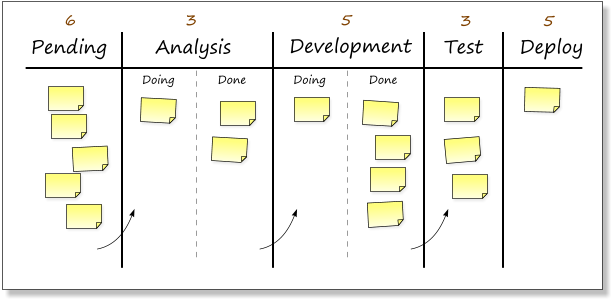
\includegraphics[width=0.9\columnwidth]{kanban-board-3} 
    \caption{Esempio di Kanban}
\end{figure}

\paragraph{Procedure}
Le procedure seguite nell'applicazione della metodologia \emph{Kanban} si appoggiano ai software aziendali rilasciati da Atlassian, ovvero JIRA e STASH.\\
In particolare, l'implementazione di una singola \emph{User Story} passa attraverso diversi passi definiti.\\
Dal lato organizzativo della stesura e realizzazione delle \emph{User Stories} e della \emph{Kanban} vera e propria, i passi da seguire sono stati i seguenti, applicati al framework JIRA:
\begin{enumerate}
	\item il Responsabile di progetto scrive la \emph{User Story};
	\item il Responsabile decide a chi assegnare l'implementazione della \emph{User Story};
	\item lo sviluppatore designato prende in carico il \emph{ticket} aperto, contrassegnandolo come "In Progress";
	\item lo sviluppatore realizza la funzionalità descritta nella \emph{User Story} della comanda;
	\item lo sviluppatore notifica l'avvenuta implementazione della funzionalità contrassegnando il ticket come "Done";
	\item il Responsabile viene notificato dell'avvenuta realizzazione e provvede all'inserimento della nuova funzionalità nel progetto.
\end{enumerate}
A questa procedura si associa anche la gestione vera e propria dei sorgenti aziendali, memorizzati in repository acceduti tramite il \emph{framework} STASH. L'implementazione di ogni \emph{feature} prevede il passaggio per vari punti, necessari alla stabilità e all'organizzazione del sistema.\\
La procedura da seguire quando si utilizza il \emph{framework} STASH è la seguente:
\begin{enumerate}
	\item prendere in carico una \emph{User Story} dal \emph{backlog};
	\item creare un nuovo \emph{branch} dall'attuale \emph{branch develop} del \emph{repository};
	\item implementare la funzionalità presa in carico, ricordandosi di effettuare \emph{commit} periodici con messaggi esplicativi del lavoro effettuato;
	\item al termine dell'implementazione, assicurarsi che i test disegnati per le unità implementate passino, così da non introdurre errori di unità nel sistema;
	\item una volta appurato che i test sono positivi, proseguire con la richiesta di \emph{pull} nel \emph{branch develop} da notificare al Responsabile del progetto.
\end{enumerate}
A questo punto si può verificare un imprevisto, ovvero che nel tempo in cui viene implementata una \emph{User Story}, il \emph{branch develop} subisca delle modifiche. Questo fatto comporta una \emph{pull} del \emph{develop} nel \emph{branch} attuale ed una conseguente risoluzione de conflitti che potrebbero venirsi a creare. Dopodiché si prosegue con la procedura:
\begin{enumerate}[resume]
	\item esaminare la risposta del Responsabile; in caso di approvazione, la procedura termina;
	\item in caso di mancata approvazione della \emph{pull request}, esaminare i punti in cui vengono alzate obiezioni da parte del Responsabile apportare le dovute modifiche al codice;
	\item ritornare al punto 4 e iterare fino ad avvenuta approvazione della \emph{pull request}.
\end{enumerate}


\subsection{Test Driven Developement}
Il modello di sviluppo \emph{Test Driven} (letteralmente tradotto in "guidato dai test") prevede che lo sviluppo di ogni unità software avvenga soltanto dopo aver scritto il corrispondente test sulla base delle specifiche dell’unità stessa.\\
Il dovere di ogni programmatore che segue questo modello è quello di scrivere il minimo quantitativo di codice necessario a far validare un test precedentemente scritto, minimizzando gli sprechi e provando la correttezza del prodotto, delegando il \emph{refactoring} stilistico ad un momento successivo, in cui si ha già un codice testato e funzionante.\\
Il motto dello sviluppo \emph{Test Driven} è appunto “Red, Green, Refactor”; la procedura da seguire prevista da questa metodologia è la seguente:
\begin{enumerate}
	\item scrivere un “singolo” test di unità che descrive una funzionalità del programma;
	\item eseguire il test, il quale dovrebbe fallire, dato che il programma non presenta ancora la \emph{feature} descritta (da qui, la fase Rossa);
	\item scrivere la quantità minima di codice necessaria far passare il test (fase Verde);
	\item eseguire il \emph{refactoring} del codice, in modo da eliminare eventuali ridondanze e superficialità;
	\item ripetere, accumulando test di unità con il passare dello sviluppo.
\end{enumerate}
 \`{E} stato scelto di utilizzare questo approccio in quanto presenta dei vantaggi significativi. Questi test permettono di individuare con precisione le specifiche del codice, e quindi il suo comportamento in base alle situazioni a cui sarà sottoposto. Ciò facilita la scrittura di un codice funzionante, più pulito, più affidabile e manutenibile.\\
La stesura di un test aiuta molto nella comprensione delle funzionalità di un modulo, evitando così errori concettuali che si potrebbero avere a priori nell'implementazione. La scrittura di un singolo test implica la piena comprensione dei metodi e delle funzionalità esposte, quindi permette di stabilire già prima della stesura di un modulo gli output attesi.\\
Il \emph{framework} AngularJS è stato creato appositamente per rendere il testing più efficiente e semplice possibile, grazie a molte funzionalità focalizzate al testing già comprese all’interno del \emph{framework}. Questa scelta è stata compiuta perché JavaScript ha una grandissima potenza espressiva, ma quasi nessun controllo da parte del compilatore, il che rende necessaria la costante presenza dei test nello sviluppo con questo linguaggio.

\subsubsection{Test di Unità}
La tipologia di test utilizzata maggiormente con questo approccio è l'insieme dei test di unità. Questa tipologia di test si prefissa di verificare il corretto funzionamento di una singola unità software. Per unità si intende normalmente il minimo componente di un programma dotato di funzionamento autonomo; a seconda del paradigma di programmazione o linguaggio di programmazione, questo può corrispondere per esempio a una singola funzione nella programmazione procedurale, o una singola classe o un singolo metodo nella programmazione a oggetti.\\
Applicando questo concetto al progetto in analisi, i test di unità scritti verificano la correttezza di ogni funzione scritta nei vari componenti del pattern \gls{mvc}\glsfirstoccur\  di AngularJS. 

\subsubsection{Test di scenario}
I test di scenario, conosciuti anche come \gls{e2e}, sono una metodologia di test utilizzata per verificare il corretto flusso di un’applicazione, se questa si comporta come pianificato dall’inizio alla fine del flusso. L’obiettivo che sta alla base della creazione di test di scenario è di identificare  le dipendenze di sistema e di assicurarsi che le informazioni (e il loro formato) siano passate correttamente tra le varie componenti del sistema.

% ----------------------------------------------------------------------------------------------------

\section{Tecnologie utilizzate}
\subsection{Tecnologie di sviluppo}
\subsubsection{AngularJS}
\begin{figure}[H] 
    \centering 
    
\includegraphics[width=0.3\columnwidth]{angularjs_logo} 
    \caption{Logo di AngularJS}
\end{figure}
AngularJS è un \emph{framework} open source JavaScript mantenuto da Google, utilizzato prevalentemente nello sviluppo di \gls{spa}\glsfirstoccur. Attraverso questo \emph{framework} è possibile aumentare le capacità del classico linguaggio \gls{html} (o simili, quali Jade), per poter realizzare applicazioni web responsive e solide. 
L’obiettivo di questo \emph{framework}, infatti, è quello di semplificare lo sviluppo ed il testing di applicazioni scritte in JavaScript, fornendo una base di librerie e direttive utili ad implementare un applicazione di architettura \gls{mvc}.\\
Come altri \emph{framework} utilizzati con lo stesso fine, una delle feature più utili ed interessanti di AngularJS è il cosiddetto \emph{“two-way data binding”}. Tramite l’utilizzo di direttive proprie del \emph{framework}, uno sviluppatore può “legare” una variabile della vista ad una particolare entità di un modello, facendo sì che i dati visualizzati rappresentino costantemente il dato aggiornato; dualmente, tramite AngularJS, se si utilizza questo legame è possibile aggiornare i dati del modello direttamente dalla vista.\\
AngularJS inoltre fornisce degli strumenti per astrarre e realizzare la comunicazione con un \gls{back-end}. Tramite AngularJS, infatti, è possibile creare un'applicazione web totalmente \gls{rest}-ful, tramite l’utilizzo delle \textbf{\$resource} e dei servizi \textbf{\$http} messi a disposizione dal \emph{framework}.

\subsubsection{Bootstrap}
\begin{figure}[htb] 
    \centering 
    
\includegraphics[width=0.4\columnwidth]{bootstrap_logo} 
    \caption{Logo di Bootstrap}
\end{figure}
\emph{Bootstrap} è una raccolta di strumenti liberi per la creazione di siti e applicazioni web. Essa contiene modelli di progettazione basati su \gls{html} e \gls{css}, sia per la tipografia, che per le varie componenti dell'interfaccia, come moduli, bottoni e navigazione, e altri componenti dell'interfaccia, così come alcune estensioni opzionali di JavaScript.
Includendo Bootstrap nella propria pagina web (sia da \gls{cdn}\glsfirstoccur\  che da codice sorgente), è possibile usufruire di tutta una serie di agevolazioni nello sviluppo di una pagina, dalla stilistica di base della pagina stessa, agli effetti di stransizione \gls{css} avanzati, al layout stesso. 
Bootstrap include una libreria \gls{css} di base con una grande varietà di classi da applicare agli elementi di \gls{html} statico, più un file \emph{JavaScript} con le funzioni \emph{jQuery} basilari di comportamento, entrambi facilmente estendibili dallo sviluppatore con file personalizzati. è una raccolta di strumenti liberi per la creazione di siti e applicazioni web. Essa contiene modelli di progettazione basati su \gls{html} e \gls{css}, sia per la tipografia, che per le varie componenti dell'interfaccia, come moduli, bottoni e navigazione, e altri componenti dell'interfaccia, così come alcune estensioni opzionali di \emph{JavaScript}.

\subsection{Strumenti di supporto ai processi}
\subsubsection{Git}
\begin{figure}[htb] 
    \centering 
    
\includegraphics[width=0.32\columnwidth]{git_logo} 
    \caption{Logo di Git}
\end{figure}
\emph{Git} è un sistema software di controllo di versione distribuito. Le funzionalità principali di \emph{Git} sono le seguenti:
\begin{itemize}
	\item \textbf{distribuzione:} \emph{Git} dà ad ogni sviluppatore una copia locale dell'intera cronologia di sviluppo, e le modifiche vengono copiate da un tale \emph{repository} a un altro. Queste modifiche vengono importate come diramazioni aggiuntive di sviluppo, e possono essere fuse allo stesso modo di una diramazione sviluppata localmente;
	\item \textbf{grande community:} considerata l’estesa community di sviluppatori che usa Git è possibile trovare diversi strumenti e \emph{plugin} che spesso semplificano il lavoro, risparmiando così tempo e risorse;
	\item \textbf{sviluppo non lineare:} \emph{Git}, attraverso il suo sistema di \emph{branching} e \emph{merging} consente lo sviluppo di codice parallelamente, su più linee che possono dividersi o unirsi.
\end{itemize}

\subsubsection{JIRA}
\begin{figure}[htb] 
    \centering 
    
\includegraphics[width=0.3\columnwidth]{JIRA_logo} 
    \caption{Logo di JIRA}
\end{figure}
Jira è un prodotto proprietario finalizzato al tracciamento dei compiti, sviluppato da Atlassian dal 2002\footcite{atlassian:jira}. Esso fornisce il tracciamento di bug, compiti e funzionalità di \emph{project managemen}t. JIRA non è un acronimo, bensì il troncamento della parola giapponese \emph{Gojira}.\\
JIRA è scritto in Java e si basa sul sistema di inversione di controllo sviluppato da Pico, su Apache OFBiz e lo stack tecnologico di WebWork 1. JIRA supporta diverse chiamate procedurali remote, quali ad esempio \gls{rest} e \gls{soap}\glsfirstoccur. JIRA si integra con i programmi di versionamento Clearcase, CVS, Git, Mercurial, Perforce, Subversion e Team Foundation Server.\\
Secondo i dati di Atlassian, JIRA viene usato nel tracciamento delle attività e nel project management da oltre 25,000 utenti in 122 paesi nel mondo. Alcune delle organizzazioni che usano JIRA sono Fedora Commons, Hibernate, Honeywell Aerospace, JBoss, Linden Lab, Skype, Spring Framework e The Apache Software Fundation.
\begin{figure}[H] 
    \centering 
    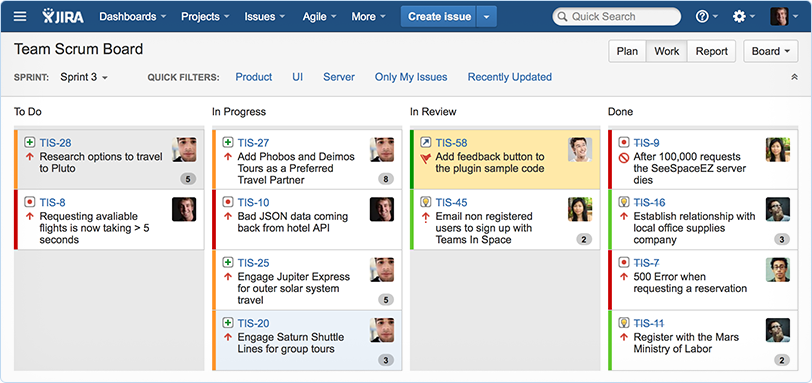
\includegraphics[width=0.9\columnwidth]{jira_kanban} 
    \caption{Esempio di schermata di una kanban di JIRA}
\end{figure}

\subsubsection{Stash}
\begin{figure}[htb] 
    \centering 
    
\includegraphics[width=0.4\columnwidth]{stash_logo} 
    \caption{Logo di Stash}
\end{figure}
STASH è un software aziendale di controllo di versionamento distribuito basato su Git.\\
Esso offre un sistema di gestione dei repository a progetto, il che predispone un naturale accompagnamento con il sistema di \emph{project management} JIRA.

\paragraph{Branching}
L’implementazione di una nuova funzionalità, secondo le strategie aziendali, viene effettuata su un nuovo \emph{branch}. Questa scelta permette lo sviluppo indipendente di più \emph{feature}, partendo da un punto comune (solitamente il \emph{branch "develop"} del \emph{repository}) e diversificando in base ai \emph{task} assegnati agli sviluppatori del team.
\begin{figure}[htb] 
    \centering 
    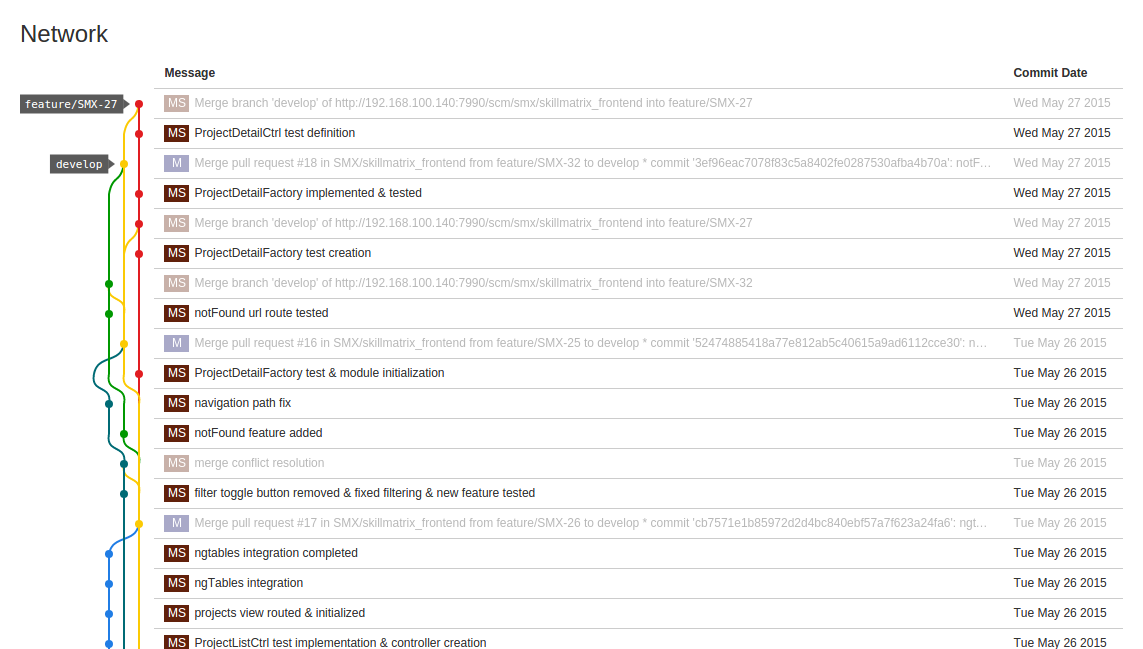
\includegraphics[width=1.0\columnwidth]{alberi} 
    \caption{\emph{Branching} e \emph{merging} in STASH}
\end{figure}

\paragraph{Pull request}
Ogniqualvolta una nuova funzionalità viene implementata, con il corrispondente completamento del \emph{ticket} dell’attività di JIRA, viene creata una \emph{“pull request”} per integrare il nuovo contenuto. Questa \emph{pull request} viene effettuata in un \emph{branch} più generale, solitamente nel \emph{“develop”} se il prodotto è ancora in via di sviluppo, oppure direttamente nel \emph{“master”} se si sta per rilasciare una nuova \emph{release} del prodotto.\\
Ogni \emph{pull request} non viene integrata finché non viene approvata dal Responsabile, il quale visiona i cambiamenti introdotti nella nuova funzionalità; egli può in ogni caso segnalare eventuali cambiamenti indesiderati allo sviluppatore e richiedere una modifica del codice.

\subsection{Ambiente di sviluppo}
\subsubsection{PhPStorm}
\begin{figure}[hb] 
    \centering 
    
\includegraphics[width=0.4\columnwidth]{phpstorm_logo} 
    \caption{Logo di PhPStorm}
\end{figure}
PhpStorm è un \gls{ide}\glsfirstoccur\  commerciale sviluppato e distribuito da JetBrains e si basa su IntelliJ IDEA.
PhpStorm fornisce un editor per \emph{PHP}, \gls{html} e JavaScript, aiutando lo sviluppatore con correzioni e segnalazioni in \emph{real time} e molte feature di refactoring del codice.\\
PhpStorm è basato su IntelliJ IDEA, che è scritto in Java. Oltre alle funzioni core dell’\gls{ide}, l’utente può estendere le funzionalità installando i numerosi plugin disponibili o scrivendone alcuni propri.\\
Oltre ad offrire un \emph{editor} responsivo ed efficiente, PhpStorm si presta molto bene per lo sviluppo di applicazioni in JavaScript, supportando i maggiori framework del linguaggio, come soprattutto AngularJS e NodeJS. 
Inoltre è possibile configurare l’\gls{ide} per l’esecuzione automatica di test scritti con Jasmine, mostrando direttamente i risultati di tali esecuzioni all’interno dell’\gls{ide} stesso, senza bisogno di un cambio di contesto e strumenti, oltre alla classica funzionalità di debugging.

\subsection{Tecnologie di Testing}
\subsubsection{Jasmine}
\begin{figure}[htb] 
    \centering 
    
\includegraphics[width=0.4\columnwidth]{jasmine_logo} 
    \caption{Logo di Jasmine}
\end{figure}
Jasmine è un \emph{framework} di testing open source per il linguaggio JavaScript. Jasmine, all’interno di un progetto in AngularJS o più in generale, può essere utilizzato sia per i test di unità dei componenti, sia per i test \gls{e2e}.\\
Jasmine si basa sulla sua facilità di comprensione dei test. Infatti, ogni test di Jasmine è diviso in blocchi di più suite. Ogni blocco riguarda una particolare componente del codice, ed ogni funzionalità testata viene correlata da una specifica descrizione del comportamento atteso.\\
Idealmente ogni statement di controllo di Jasmine dovrebbe testare non più di una funzione del codice, così da rendere i controlli maggiormente atomici. Per aiutare lo sviluppatore nella scrittura dei test, Jasmine presenta al suo interno una grande quantità di costrutti di confronto, che spaziano sui diversi tipi di dato che si possono incontrare, lasciando comunque allo sviluppatore il modo di creare confronti personalizzati.\\
Usato insieme ad AngularJS, Jasmine arricchisce ulteriormente le sue potenzialità, in quanto AngularJS comprende un modulo apposito scritto per il testing, ovvero \emph{angular-mocks}. In questo modulo, da includere in Jasmine, troviamo i costruttori di ogni componente di Angular, con cui iniettare le varie componenti mockate quando ne abbiamo l’esigenza, come ad esempio nel test di un controller che dipende da uno o più servizi, più altre componenti utili allo sviluppatore.\\
Per quanto riguarda i test \gls{e2e}, Jasmine contiene al suo interno vari strumenti di simulazione di input utente, quali ad esempio il click su un elemento o l’inserimento di testo in una casella. Attraverso l’uso di questi strumenti, è possibile simulare vari scenari di interazione con le varie funzionalità del sistema, andando quindi a testare il corretto funzionamento delle varie unità. 
Questo si ottiene sfruttando di browser driver come \emph{Selenium}, i quali automatizzano l’interazione con i vari \emph{browser}.

\subsection{Strumenti di Automazione}
\subsubsection{Grunt}
\begin{figure}[htb] 
    \centering 
    
\includegraphics[width=0.3\columnwidth]{grunt_logo} 
    \caption{Logo di Grunt}
\end{figure}
Grunt è un gestore ed un esecutore di attività JavaScript. Utilizzato soprattutto per l’automazione di attività come \emph{minificazione}, compilazione, test di unità, di scenario, ecc., aiuta lo sviluppatore soprattutto nella creazione di applicazioni \emph{client side}, aumentando l’efficienza nello sviluppo.\\ 
A seconda delle esigenze e delle possibilità hardware, infatti, Grunt può essere configurato in modo che vengano eseguiti certi script ad ogni modifica di un file, o solo di alcuni. Si può quindi ricaricare un \emph{webserver} alla modifica di un file \gls{html} o eseguire un certo test di unità alla modifica di un file JavaScript, il tutto assolutamente automatizzato.\\
Inoltre Grunt e la sua community sono in continuo sviluppo; ci sono molti sviluppatori che scrivono attorno a questa tecnologia, creando \emph{plugin} da utilizzare per automatizzare anche il sistema di configurazione di Grunt, per adattarsi ai vari \emph{framework} utilizzati durante lo sviluppo.

\subsubsection{Karma}
\begin{figure}[htb] 
    \centering 
    
\includegraphics[width=0.4\columnwidth]{karma_logo} 
    \caption{Logo di Karma}
\end{figure}
Karma, precedentemente conosciuto come \emph{Testacular}, è un ambiente creato per il lancio e la gestione dei test in ambiente JavaScript.\\
Karma supporta diversi \emph{framework} di testing, inoltre è compatibile con i maggiori browser per assicurare che l’ambiente utilizzato per il testing sia funzionante in tutti i casi.\\
L’unico compito che ha lo sviluppatore, per poter utilizzare Karma, è (oltre all’installazione del \emph{client} e dei \emph{plugin} necessari) creare e personalizzare il file di configurazione di Karma, la cui struttura viene creata in automatico con un comando del client da terminale.\\
All’interno del file di configurazione, lo sviluppatore può configurare tutti gli aspetti dell’esecuzione dei test, dai browser utilizzati alla selezione di quali test eseguire, in una esecuzione singola o ad aggiornamento dei file. 
Oltre ad eseguire i test che vengono specificati nei path del file di configurazione, Karma offre anche altre funzionalità interessanti che si appoggiano sui test scritti. Una di queste funzionalità è la generazione automatica di un file di \emph{html} statico in cui vengono mostrate le singole metriche di coverage di ogni file e in media per il progetto. Le metriche di copertura generate automaticamente con il \emph{plugin} \emph{coverage} di Karma sono:
\begin{itemize}
	\item line coverage;
	\item statement coverage;
	\item branch coverage;
	\item function coverage.
\end{itemize}
Nella “vista” che viene creata dal \emph{plugin}, è possibile visualizzare quali linee non sono eventualmente coperte dai test, quali branch e quali funzioni, su cui quindi andare ad intervenire o meno per aumentare la copertura, o per verificare che ogni funzionalità sia effettivamente implementata e testata.

\subsubsection{NPM}
\begin{figure}[htb] 
    \centering 
    
\includegraphics[width=0.4\columnwidth]{npm_logo} 
    \caption{Logo di NPM}
\end{figure}
Acronimo di \emph{Node Package Manager}. Come da definizione, \gls{npm}\glsfirstoccur\  è un gestore di pacchetti e moduli JavaScript, basato su Node.js.\\ 
Tramite \gls{npm} è possibile cercare ed installare localmente ad un progetto o globalmente una grande serie di utilità pubblicate nel registro stesso di \gls{npm}. Oltre a questo, è possibile gestire ed aggiornare facilmente ogni pacchetto installato tramite semplici comandi da terminale.\\
La gestione dei pacchetti di npm consente di suddividere i moduli in funzionalità, per garantire così il riutilizzo atomico e una maggiore manutenibilità dei singoli file, così come la condivisione con altri sviluppatori attraverso il registro \gls{npm}. 

\subsubsection{Protractor}
\begin{figure}[htb] 
    \centering 
    
\includegraphics[width=0.4\columnwidth]{protractor_logo} 
    \caption{Logo di Protractor}
\end{figure}
Protractor è un \emph{framework} utilizzato per eseguire test \emph{e2e}, pensato soprattutto per la compatibilità con AngularJS. Protractor è un \emph{framework} scritto in NodeJS, mentre la sua base e l’interazione con i vari browser è mediata da WebDriverJS.\\
Questo \emph{framework} permette di eseguire i comandi pensati e scritti nei test \gls{e2e}. Ovvero, permette di simulare il comportamento di un utente con una certa applicazione web, verificando che gli output attesi di una certa applicazione ad un certo comportamento utente, siano quelli previsti. Tramite l’utilizzo di \emph{Selenium} WebDriverJS, questo procedimento di testing viene completamente automatizzato; si riescono a replicare le tipiche azioni di un utente e Protractor analizza ogni risposta dell’applicazione e la confronta con le attese.\\
Alla fine di ogni test suite, ci vengono presentati i risultati dell’esecuzione dei test e, se ci sono, quali statement hanno provocato un errore.

